\section{Identificação de genes alvos de DREBs}
   \frame{\justifying
    \frametitle{Identificação de genes alvos de DREBs}
		Para identificar os genes alvos de DREBs \cite{Wang2009} criaram a seguinte estratégia:
		
		 	
	}
	
   \frame{\justifying
    \frametitle{Identificação de genes alvos de DREBs}
		\begin{figure}[htb!]
		    \centering
		    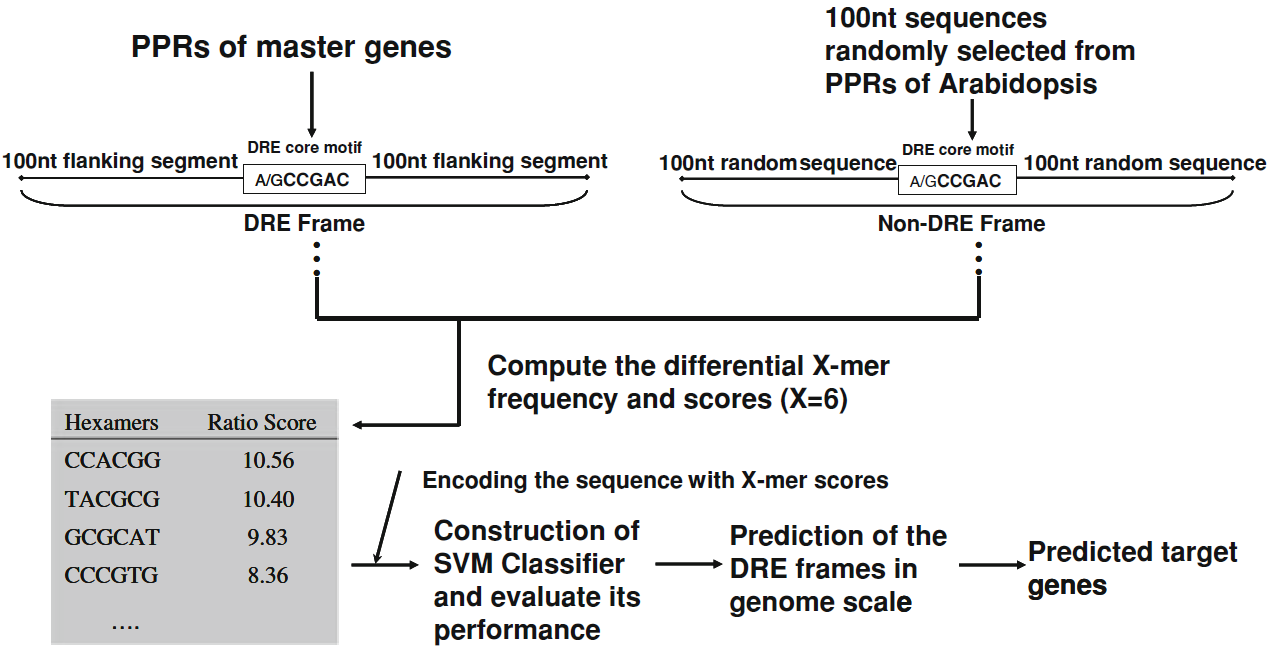
\includegraphics[scale=0.33]{./imagens/esq_DREB_find.png}
		    \caption{Busca DREBs}
		    \label{fig:esq_DREB_find}
		\end{figure}		    	
	}

   \frame{\justifying
    \frametitle{Identificação de genes alvos de DREBs}
		\begin{itemize}
			\item Achar a frequência em ambos os conjuntos $F{p}\{h\} e F_{n}\{h\}$.
			\item Calcular a razão $ R\{h\} = \frac{F{p}\{h\}}{F_{n}\{h\}}$
			\item Os DFS e nDFS recebem identificação de (+1) e (-1), respectivamente.
			\item SVM é treinada para distinguir entre DFS e nDFS.
		\end{itemize}	
	}